\PassOptionsToPackage{unicode=true}{hyperref} % options for packages loaded elsewhere
\PassOptionsToPackage{hyphens}{url}
%
\documentclass[]{article}
\usepackage{lmodern}
\usepackage{amssymb,amsmath}
\usepackage{ifxetex,ifluatex}
\usepackage{fixltx2e} % provides \textsubscript
\ifnum 0\ifxetex 1\fi\ifluatex 1\fi=0 % if pdftex
  \usepackage[T1]{fontenc}
  \usepackage[utf8]{inputenc}
  \usepackage{textcomp} % provides euro and other symbols
\else % if luatex or xelatex
  \usepackage{unicode-math}
  \defaultfontfeatures{Ligatures=TeX,Scale=MatchLowercase}
\fi
% use upquote if available, for straight quotes in verbatim environments
\IfFileExists{upquote.sty}{\usepackage{upquote}}{}
% use microtype if available
\IfFileExists{microtype.sty}{%
\usepackage[]{microtype}
\UseMicrotypeSet[protrusion]{basicmath} % disable protrusion for tt fonts
}{}
\IfFileExists{parskip.sty}{%
\usepackage{parskip}
}{% else
\setlength{\parindent}{0pt}
\setlength{\parskip}{6pt plus 2pt minus 1pt}
}
\usepackage{hyperref}
\hypersetup{
            pdftitle={Re-analysis of GSE160729 adipocyte snRNAseq},
            pdfauthor={Dave Bridges},
            pdfborder={0 0 0},
            breaklinks=true}
\urlstyle{same}  % don't use monospace font for urls
\usepackage[margin=1in]{geometry}
\usepackage{color}
\usepackage{fancyvrb}
\newcommand{\VerbBar}{|}
\newcommand{\VERB}{\Verb[commandchars=\\\{\}]}
\DefineVerbatimEnvironment{Highlighting}{Verbatim}{commandchars=\\\{\}}
% Add ',fontsize=\small' for more characters per line
\usepackage{framed}
\definecolor{shadecolor}{RGB}{248,248,248}
\newenvironment{Shaded}{\begin{snugshade}}{\end{snugshade}}
\newcommand{\AlertTok}[1]{\textcolor[rgb]{0.94,0.16,0.16}{#1}}
\newcommand{\AnnotationTok}[1]{\textcolor[rgb]{0.56,0.35,0.01}{\textbf{\textit{#1}}}}
\newcommand{\AttributeTok}[1]{\textcolor[rgb]{0.77,0.63,0.00}{#1}}
\newcommand{\BaseNTok}[1]{\textcolor[rgb]{0.00,0.00,0.81}{#1}}
\newcommand{\BuiltInTok}[1]{#1}
\newcommand{\CharTok}[1]{\textcolor[rgb]{0.31,0.60,0.02}{#1}}
\newcommand{\CommentTok}[1]{\textcolor[rgb]{0.56,0.35,0.01}{\textit{#1}}}
\newcommand{\CommentVarTok}[1]{\textcolor[rgb]{0.56,0.35,0.01}{\textbf{\textit{#1}}}}
\newcommand{\ConstantTok}[1]{\textcolor[rgb]{0.00,0.00,0.00}{#1}}
\newcommand{\ControlFlowTok}[1]{\textcolor[rgb]{0.13,0.29,0.53}{\textbf{#1}}}
\newcommand{\DataTypeTok}[1]{\textcolor[rgb]{0.13,0.29,0.53}{#1}}
\newcommand{\DecValTok}[1]{\textcolor[rgb]{0.00,0.00,0.81}{#1}}
\newcommand{\DocumentationTok}[1]{\textcolor[rgb]{0.56,0.35,0.01}{\textbf{\textit{#1}}}}
\newcommand{\ErrorTok}[1]{\textcolor[rgb]{0.64,0.00,0.00}{\textbf{#1}}}
\newcommand{\ExtensionTok}[1]{#1}
\newcommand{\FloatTok}[1]{\textcolor[rgb]{0.00,0.00,0.81}{#1}}
\newcommand{\FunctionTok}[1]{\textcolor[rgb]{0.00,0.00,0.00}{#1}}
\newcommand{\ImportTok}[1]{#1}
\newcommand{\InformationTok}[1]{\textcolor[rgb]{0.56,0.35,0.01}{\textbf{\textit{#1}}}}
\newcommand{\KeywordTok}[1]{\textcolor[rgb]{0.13,0.29,0.53}{\textbf{#1}}}
\newcommand{\NormalTok}[1]{#1}
\newcommand{\OperatorTok}[1]{\textcolor[rgb]{0.81,0.36,0.00}{\textbf{#1}}}
\newcommand{\OtherTok}[1]{\textcolor[rgb]{0.56,0.35,0.01}{#1}}
\newcommand{\PreprocessorTok}[1]{\textcolor[rgb]{0.56,0.35,0.01}{\textit{#1}}}
\newcommand{\RegionMarkerTok}[1]{#1}
\newcommand{\SpecialCharTok}[1]{\textcolor[rgb]{0.00,0.00,0.00}{#1}}
\newcommand{\SpecialStringTok}[1]{\textcolor[rgb]{0.31,0.60,0.02}{#1}}
\newcommand{\StringTok}[1]{\textcolor[rgb]{0.31,0.60,0.02}{#1}}
\newcommand{\VariableTok}[1]{\textcolor[rgb]{0.00,0.00,0.00}{#1}}
\newcommand{\VerbatimStringTok}[1]{\textcolor[rgb]{0.31,0.60,0.02}{#1}}
\newcommand{\WarningTok}[1]{\textcolor[rgb]{0.56,0.35,0.01}{\textbf{\textit{#1}}}}
\usepackage{longtable,booktabs}
% Fix footnotes in tables (requires footnote package)
\IfFileExists{footnote.sty}{\usepackage{footnote}\makesavenoteenv{longtable}}{}
\usepackage{graphicx,grffile}
\makeatletter
\def\maxwidth{\ifdim\Gin@nat@width>\linewidth\linewidth\else\Gin@nat@width\fi}
\def\maxheight{\ifdim\Gin@nat@height>\textheight\textheight\else\Gin@nat@height\fi}
\makeatother
% Scale images if necessary, so that they will not overflow the page
% margins by default, and it is still possible to overwrite the defaults
% using explicit options in \includegraphics[width, height, ...]{}
\setkeys{Gin}{width=\maxwidth,height=\maxheight,keepaspectratio}
\setlength{\emergencystretch}{3em}  % prevent overfull lines
\providecommand{\tightlist}{%
  \setlength{\itemsep}{0pt}\setlength{\parskip}{0pt}}
\setcounter{secnumdepth}{5}
% Redefines (sub)paragraphs to behave more like sections
\ifx\paragraph\undefined\else
\let\oldparagraph\paragraph
\renewcommand{\paragraph}[1]{\oldparagraph{#1}\mbox{}}
\fi
\ifx\subparagraph\undefined\else
\let\oldsubparagraph\subparagraph
\renewcommand{\subparagraph}[1]{\oldsubparagraph{#1}\mbox{}}
\fi

% set default figure placement to htbp
\makeatletter
\def\fps@figure{htbp}
\makeatother


\title{Re-analysis of GSE160729 adipocyte snRNAseq}
\author{Dave Bridges}
\date{May 27, 2021}

\begin{document}
\maketitle

{
\setcounter{tocdepth}{2}
\tableofcontents
}
\hypertarget{purpose}{%
\section{Purpose}\label{purpose}}

To reanalyse a single cell RNAseq study on adipocyte tissue.

\hypertarget{experimental-details}{%
\section{Experimental Details}\label{experimental-details}}

Savari et al used HFD-induced obesity and then did single nuclei
isolation.

\hypertarget{raw-data}{%
\section{Raw Data}\label{raw-data}}

Savari et al shared code and Rds friles for annotated adipocytes at
\url{https://osf.io/tsjqc/} and
\url{https://github.com/JesperGrud/snRNAseq_eWAT}

Loaded in the annotated Rds file from OSF, renamed as
`\texttt{input.rds.adipocytes}

Followed the Seurat clustering protocol
\url{https://satijalab.org/seurat/articles/pbmc3k_tutorial.html}

\hypertarget{highly-variable-features-in-adipocytes}{%
\subsection{Highly Variable Features in
Adipocytes}\label{highly-variable-features-in-adipocytes}}

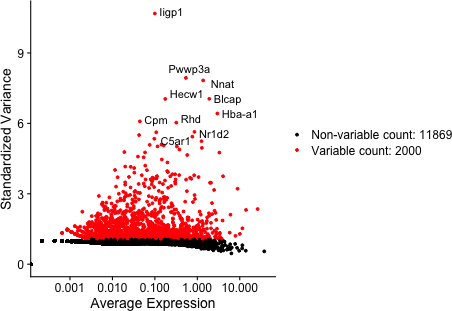
\includegraphics{figures/GSE160729-variable-features-1.png}

\hypertarget{scaling-and-dimensional-reduction}{%
\section{Scaling and Dimensional
Reduction}\label{scaling-and-dimensional-reduction}}

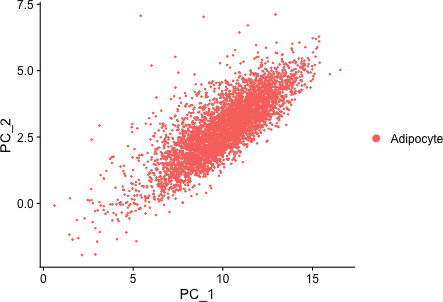
\includegraphics{figures/GSE160729-scale-pca-1.png}
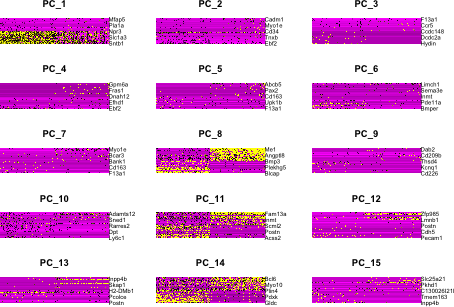
\includegraphics{figures/GSE160729-scale-pca-2.png}
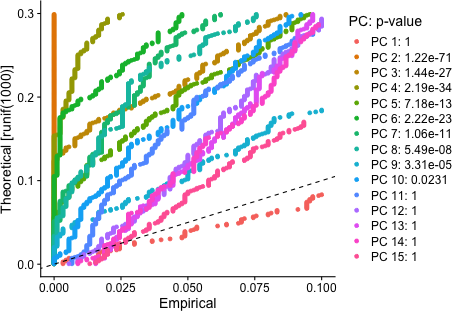
\includegraphics{figures/GSE160729-scale-pca-3.png}
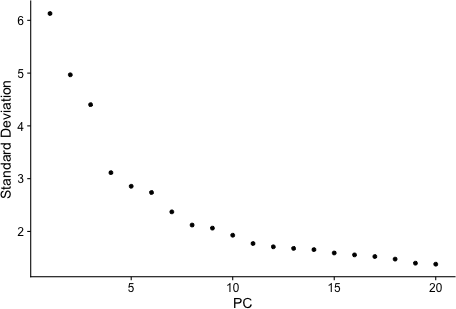
\includegraphics{figures/GSE160729-scale-pca-4.png}

\hypertarget{cell-clustering}{%
\subsection{Cell Clustering}\label{cell-clustering}}

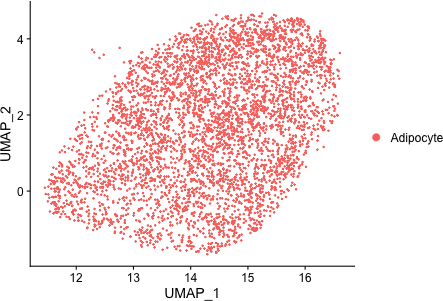
\includegraphics{figures/GSE160729-clustering-1.png}
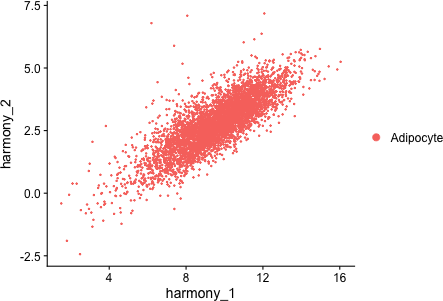
\includegraphics{figures/GSE160729-clustering-2.png}
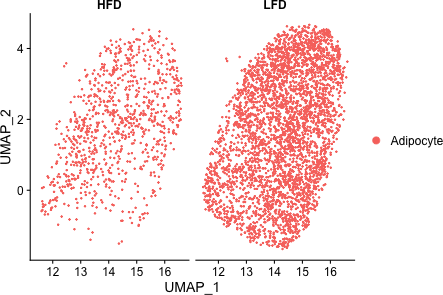
\includegraphics{figures/GSE160729-clustering-3.png}
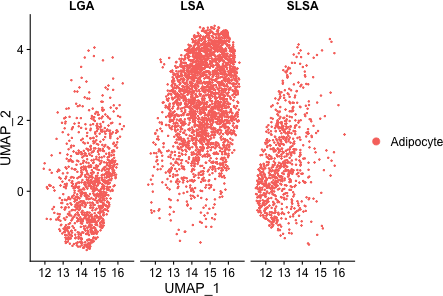
\includegraphics{figures/GSE160729-clustering-4.png}

\hypertarget{cluster-biomarkers}{%
\subsection{Cluster Biomarkers}\label{cluster-biomarkers}}

\hypertarget{differential-expresion}{%
\section{Differential Expresion}\label{differential-expresion}}

\begin{verbatim}
##            p_val avg_log2FC pct.1 pct.2 p_val_adj
## Svs5   9.94e-189       7.32 0.576 0.010 1.38e-184
## Svs4   1.76e-189       6.05 0.576 0.006 2.44e-185
## Svs6   1.10e-189       4.45 0.576 0.005 1.52e-185
## Acaca   0.00e+00       3.75 0.964 0.517  0.00e+00
## Spinkl 3.60e-186       3.11 0.566 0.001 4.99e-182
## Thrsp  2.87e-289       2.99 0.842 0.185 3.98e-285
\end{verbatim}

\begin{longtable}[]{@{}lrrrrr@{}}
\caption{HFD-Differentially Expressed Transcription Factors in
Adipocytes}\tabularnewline
\toprule
Gene & p\_val & avg\_log2FC & pct.1 & pct.2 & p\_val\_adj\tabularnewline
\midrule
\endfirsthead
\toprule
Gene & p\_val & avg\_log2FC & pct.1 & pct.2 & p\_val\_adj\tabularnewline
\midrule
\endhead
Esrrg & 0.000 & -0.728 & 0.104 & 0.399 & 0.000\tabularnewline
Zfp423 & 0.000 & -0.520 & 0.452 & 0.637 & 0.000\tabularnewline
Sox5 & 0.000 & -0.511 & 0.625 & 0.768 & 0.000\tabularnewline
Atf7ip & 0.000 & -0.481 & 0.294 & 0.509 & 0.000\tabularnewline
Klf13 & 0.000 & -0.446 & 0.565 & 0.734 & 0.000\tabularnewline
Hivep2 & 0.000 & -0.400 & 0.747 & 0.852 & 0.000\tabularnewline
Mnat1 & 0.000 & -0.381 & 0.408 & 0.570 & 0.000\tabularnewline
Phf8 & 0.000 & -0.376 & 0.221 & 0.410 & 0.000\tabularnewline
Foxp1 & 0.000 & -0.295 & 0.601 & 0.713 & 0.000\tabularnewline
Enpp2 & 0.004 & -0.262 & 0.364 & 0.405 & 1.000\tabularnewline
Hivep3 & 0.000 & -0.257 & 0.296 & 0.425 & 0.000\tabularnewline
Ar & 0.000 & 0.281 & 0.383 & 0.289 & 0.000\tabularnewline
Nr3c1 & 0.000 & 0.325 & 0.366 & 0.207 & 0.000\tabularnewline
Esr1 & 0.000 & 0.327 & 0.345 & 0.235 & 0.000\tabularnewline
Ppargc1b & 0.000 & 0.352 & 0.343 & 0.203 & 0.000\tabularnewline
Tcf7l2 & 0.000 & 0.410 & 0.745 & 0.655 & 0.000\tabularnewline
Bcl6 & 0.000 & 0.450 & 0.493 & 0.426 & 0.001\tabularnewline
Nfib & 0.000 & 0.453 & 0.915 & 0.847 & 0.000\tabularnewline
Zfpm2 & 0.000 & 0.540 & 0.478 & 0.256 & 0.000\tabularnewline
Sox6 & 0.000 & 0.561 & 0.662 & 0.461 & 0.000\tabularnewline
Ebf2 & 0.000 & 0.738 & 0.524 & 0.239 & 0.000\tabularnewline
Ank2 & 0.000 & 1.086 & 0.796 & 0.482 & 0.000\tabularnewline
Pparg & 0.000 & 1.254 & 0.963 & 0.839 & 0.000\tabularnewline
Nfia & 0.000 & 1.712 & 0.988 & 0.877 & 0.000\tabularnewline
Thrsp & 0.000 & 2.988 & 0.842 & 0.185 & 0.000\tabularnewline
\bottomrule
\end{longtable}

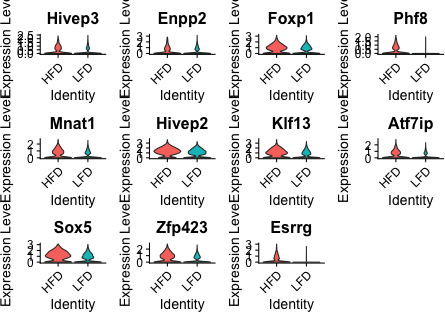
\includegraphics{figures/GSE160729-de-by-hfd-1.png}
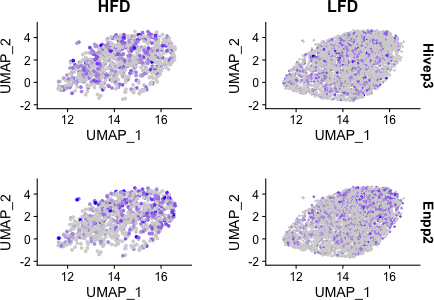
\includegraphics{figures/GSE160729-de-by-hfd-2.png}

\hypertarget{session-information}{%
\section{Session Information}\label{session-information}}

\begin{Shaded}
\begin{Highlighting}[]
\KeywordTok{sessionInfo}\NormalTok{()}
\end{Highlighting}
\end{Shaded}

\begin{verbatim}
## R version 4.0.2 (2020-06-22)
## Platform: x86_64-apple-darwin17.0 (64-bit)
## Running under: macOS  10.16
## 
## Matrix products: default
## BLAS:   /Library/Frameworks/R.framework/Versions/4.0/Resources/lib/libRblas.dylib
## LAPACK: /Library/Frameworks/R.framework/Versions/4.0/Resources/lib/libRlapack.dylib
## 
## locale:
## [1] en_US.UTF-8/en_US.UTF-8/en_US.UTF-8/C/en_US.UTF-8/en_US.UTF-8
## 
## attached base packages:
## [1] stats     graphics  grDevices utils     datasets  methods   base     
## 
## other attached packages:
## [1] ggplot2_3.3.3      rvest_1.0.0        SeuratObject_4.0.1 Seurat_4.0.2      
## [5] umap_0.2.7.0       tibble_3.1.2       dplyr_1.0.6        tidyr_1.1.3       
## [9] knitr_1.33        
## 
## loaded via a namespace (and not attached):
##   [1] Rtsne_0.15            colorspace_2.0-1      deldir_0.2-10        
##   [4] ellipsis_0.3.2        ggridges_0.5.3        spatstat.data_2.1-0  
##   [7] farver_2.1.0          leiden_0.3.7          listenv_0.8.0        
##  [10] ggrepel_0.9.1         RSpectra_0.16-0       fansi_0.5.0          
##  [13] xml2_1.3.2            codetools_0.2-18      splines_4.0.2        
##  [16] polyclip_1.10-0       jsonlite_1.7.2        ica_1.0-2            
##  [19] cluster_2.1.2         png_0.1-7             uwot_0.1.10          
##  [22] shiny_1.6.0           sctransform_0.3.2     spatstat.sparse_2.0-0
##  [25] compiler_4.0.2        httr_1.4.2            assertthat_0.2.1     
##  [28] Matrix_1.3-3          fastmap_1.1.0         lazyeval_0.2.2       
##  [31] limma_3.46.0          later_1.2.0           htmltools_0.5.1.1    
##  [34] tools_4.0.2           igraph_1.2.6          gtable_0.3.0         
##  [37] glue_1.4.2            RANN_2.6.1            reshape2_1.4.4       
##  [40] Rcpp_1.0.6            scattermore_0.7       vctrs_0.3.8          
##  [43] nlme_3.1-152          lmtest_0.9-38         xfun_0.23            
##  [46] stringr_1.4.0         globals_0.14.0        mime_0.10            
##  [49] miniUI_0.1.1.1        lifecycle_1.0.0       irlba_2.3.3          
##  [52] goftest_1.2-2         future_1.21.0         MASS_7.3-54          
##  [55] zoo_1.8-9             scales_1.1.1          spatstat.core_2.1-2  
##  [58] promises_1.2.0.1      spatstat.utils_2.1-0  parallel_4.0.2       
##  [61] RColorBrewer_1.1-2    curl_4.3.1            yaml_2.2.1           
##  [64] reticulate_1.20       pbapply_1.4-3         gridExtra_2.3        
##  [67] rpart_4.1-15          stringi_1.6.2         highr_0.9            
##  [70] rlang_0.4.11          pkgconfig_2.0.3       matrixStats_0.58.0   
##  [73] evaluate_0.14         lattice_0.20-44       ROCR_1.0-11          
##  [76] purrr_0.3.4           tensor_1.5            labeling_0.4.2       
##  [79] patchwork_1.1.1       htmlwidgets_1.5.3     cowplot_1.1.1        
##  [82] tidyselect_1.1.1      parallelly_1.25.0     RcppAnnoy_0.0.18     
##  [85] plyr_1.8.6            magrittr_2.0.1        R6_2.5.0             
##  [88] magick_2.7.2          generics_0.1.0        DBI_1.1.1            
##  [91] withr_2.4.2           pillar_1.6.1          mgcv_1.8-35          
##  [94] fitdistrplus_1.1-3    survival_3.2-11       abind_1.4-5          
##  [97] future.apply_1.7.0    crayon_1.4.1          KernSmooth_2.23-20   
## [100] utf8_1.2.1            spatstat.geom_2.1-0   plotly_4.9.3         
## [103] rmarkdown_2.8         grid_4.0.2            data.table_1.14.0    
## [106] digest_0.6.27         xtable_1.8-4          httpuv_1.6.1         
## [109] openssl_1.4.4         munsell_0.5.0         viridisLite_0.4.0    
## [112] askpass_1.1
\end{verbatim}

\end{document}
